%\documentclass[•]{•}10pt,conference,compsocconf,letterpaper]{IEEEtran}
\documentclass[10pt,pdftex,a4paper]{article}%
\pdfoutput=1
\usepackage{graphicx}
%\usepackage{enumitem}
%\setlist{nolistsep}
\usepackage[margin=1in]{geometry}
\usepackage{cite}
%\usepackage{authblk}
\usepackage{multicol}
\usepackage{color}
\usepackage{algorithmic}
\usepackage{listings}
\newcommand{\commentaj}[1]{{\color{blue} \textit{aj: #1}}}
\newcommand{\commentsu}[1]{{\color{green} \textit{su: #1}}}
\newcommand{\commentdk}[1]{{\color{red} \textit{dk: #1}}}
% ---
% Make bibliography use section numbering
% https://tex.stackexchange.com/questions/23012/how-can-i-include-bibliography-into-numbering
%\usepackage{etoolbox}
%\patchcmd{\thebibliography}{*}{}{}{}

% ---
\begin{document}


\title{Implementation of a Non-Blocking Binary Search Tree in C++\\Final Report}
\author{Akshay Jajoo, Devesh Kumar Singh, Sergei Uversky}
%\affil{Purdue University}
\date{May 05, 2016}
\maketitle
%%%%%%%%%%%%%%%%%%%%%%%%%%%%%%%%%%%%%%%%%%%%%%%%%%%%%%%%%%%%%%%%%%%%%%%%%%%%%%%%
\pagenumbering{arabic}\setcounter{page}{1}
\begin{multicols}{2}
\section{Introduction}
Sequential data structures are unable to take advantage of the unique capabilities of modern shared-memory multiprocessor machines, leading to poorer-than-optimal performance. This has brought about a need for concurrent data structures in shared memory, through which threads can communicate and synchronize effectively, allowing programs to harness the power of concurrent computing. \cite{shavit} In this course project, we aim to implement a non-blocking  concurrent version of one of the most common data structures: the binary search tree.

\section{Motivation}
Throughout the course of this semester, we have studied various approaches to making concurrent data structures like stacks, queues, sets etc. satisfying both lock-based and lock-free liveness guarantees.  Although it is relatively simple to reason about and implement lock-based concurrent data structures, they come with a number of drawbacks: most importantly, they introduce a \textit{sequential bottleneck}; further, in the context of this course, they are useless for anything but the most naive (crash-free) failure model, as a process that holds a lock and crashes while in the lock's critical section renders progress impossible.  Thus, when dealing with distributed systems, we ideally seek data structures that satisfy non-blocking liveness guarantees such as lock-freedom and wait-freedom, as these are more applicable in a realistic distributed setting with non-trivial failure models.

There has been a good amount of progress on making non-blocking implementations of simple data structures like arrays, stacks and queues, but very little for binary search trees. To this end, we seek to implement a non-blocking version of a binary search tree in a non-managed language (C++). As far as we know, no concrete implementation for non-blocking BSTs exists in a non-managed language.  We hope that by tackling such an implementation in a non-managed language, we can identify some non-trivial implementation-specific pain points that are not identified in the theoretical discussions, as well as benchmark performance. 

\section{Related Work}

The bulk of our project is aimed at implementing the theoretical non-blocking binary search tree found in the work by Ellen, Fatourou, Ruppert and van Breugel.\cite{ellen10}  In this work, Ellen et al. outline the theory and provide the pseudo-code for the first known implementation of a non-blocking binary search tree.  Additionally, they provide a proof sketch for the correctness of their work.  However, they do not actually have an implementation of their work available in the paper, and thus there are no benchmarks comparing this implementation to other state-of-the-art implementations, either sequential or lock-based concurrent.

Lock-based concurrent BSTs have been tackled in theory as early as 1978; see the work done by Guibas and Sedgewick\cite{guibas78} and Kung and Lehman\cite{kung80}.  Implementations of these lock-based BSTs appear in both unbalanced and balanced forms; one notable example of the latter is the Java implementation by Bronson, Casper, Chafi and Olukotun\cite{bronson09}.

Non-blocking concurrent BSTs have been described by other researchers since Ellen's work.  One example is the work by Chatterjee, Nguyen and Tsigas\cite{chatterjee14}, which includes an analysis of computational complexity.

\section{Algorithms} 
\subsection{Problem Formulation}
As stated above, we aimed to provide a C or C++ implementation of the non-blocking binary search tree described in the work of Ellen et al. The crux of the algorithm described in that work is a state setting for each node -- if one process is in the middle of running an update operation on a node, other concurrent processes can tell how far along that process is based on the bits of the state setting.  The \textsc{Find} operation is read-only and does not change any child pointers in the node, and thus can be safely run concurrently (i.e. it need not CAS this state setting).  The \textsc{Insert} and \textsc{Delete} operations first start by marking the nodes which might get affected by the operations, help other concurrent operations on which the operation might be waiting for complete, and then proceed to perform the actual insert and delete. Marking the nodes allows other processes to "pick up the slack" for any stuck/crashed processes, providing a non-blocking liveness guarantee.

The implementation we aimed at involved gathering a deep understanding of both the theory and pseudo-code given in the paper and the practice of non-blocking concurrent programming in C and C++ (e.g. the interface to dealing with CAS cross-platform, etc.)  We expected that this in itself will be no easy task, and that it would form the bulk of our work.  To this end, we began by handling the comparatively simpler \textsc{Insert} and \textsc{Find} operations.  We hope to continue by modifying the \textsc{Insert} operation to maintain at least a relaxed semblance of balance in the tree.  Implementing \textsc{Delete} is unfortunately unlikely, as it requires an understanding of concurrent memory management and garbage collection beyond the scope of this project.

\subsection{Overview}

As in the work by Ellen et al, we consider a \textit{leaf-oriented BST}, where nodes with relevant data are found in the leaves of the tree.  The keys stored in the internal nodes of the tree are used to direct the search operation that the algorithm conducts to find where to insert a tree.  We maintain the invariant that for each internal node $n$ with children $n_l := x\rightarrow left$ and $n_r := x\rightarrow right$, $\textsc{Key}(n_l) < \textsc{Key}(n) \leq \textsc{Key}(n_r)$.  (In the original algorithm described by Ellen et al, the keys of internal nodes could potentially not correspond to existing keys in the tree due to deletions; as we do not yet support deletions, our internal node key set is equal to our leaf key set.)  The \textsc{Find$(k)$} operation is comparable to its sequential implementation.  An \textsc{Insert$(k)$} operation, if it is successful, replaces a leaf with a subtree, i.e. an internal node with two children (see Figure 1, pulled from Ellen's paper).

\begin{center}
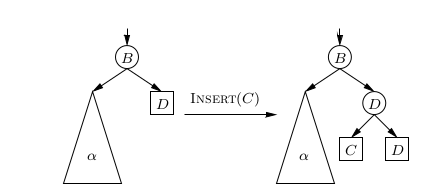
\includegraphics[width=0.5\textwidth]{insert.png}
Figure 1: \textsc{Insert$(k)$} (credit to Ellen et al.)
\end{center}

\subsection{Sequential BST}
We implemented a naive sequential version of a BST for benchmarking purposes.  This implementation leverages the interface used by the non-blocking implementation but avoids the use of CAS as well as data structures specific to the non-blocking implementation.  The implementation is relatively trivial and does not differ appreciably from any standard BST implementation that can be found in any relevant reference material.

\subsubsection{Transactional memory-based extension}
As an additional benchmark, we have leveraged our naive sequential implementation to make a concurrent leaf-oriented BST by using the transactional memory constructs of GCC. Recall from class that \textit{transactional memory} is an approach that attempts to combine the performance benefits of concurrency with the simplicity of sequential programming.  In this approach, transactions consisting of one or more operations run in isolation and either commit (pushing all of their operations atomically) or abort (discarding the potential changes made by the operations), resulting in a consistent view of memory.

GCC provides support for transactional memory by supplying some annotations and some wrappers around existing sequential code.  This is straightforward to implement and again does not need an appreciable amount of elaboration; the only thing to note is that the non-thread-safe portions of the sequential code are wrapped in \texttt{\_\_transaction\_atomic} blocks.

\subsubsection{Lock-based extension}
For benchmarking, we will also extend this sequential implementation with locks to make a simplistic blocking thread-safe implementation.

\subsection{Non-blocking BST}
As of C++11, the C++ standard library provides support for atomic objects via the \texttt{<atomic>} library.  Instead of using a simple \texttt{foo} object, we can instead use an \texttt{atomic<foo>} to guarantee memory ordering in multithreaded contexts.  Crucially, these \texttt{atomic<foo>} objects support a \texttt{compare\_exchange\_strong}\footnote{There is also a \texttt{compare\_exchange\_weak} variant, which is potentially faster at the expense of allowing spurious failures.} operation, which is a platform-independent implementation of CAS.\footnote{As far as the authors understand, the C++ STL CAS implementation uses a hardware CAS where available for 8-byte words or smaller, and uses mutexes to emulate CAS otherwise.  More investigation into the implementation is necessary for future work.}

The Ellen paper describes an approach in which update operations CAS on a node's status to make progress -- in their work, the status is one of \textsc{Clean} (no operations pending), \textsc{Mark} (child node currently being deleted), \textsc{IFlag} (node currently being inserted) or \textsc{DFlag} (node currently being deleted).  The status is used to ensure that the internal state of the tree is consistent during concurrent operations.  Nodes progress through the statuses via CAS, ensuring that at most one process is able to further a node's status; because of the internal consistency this imposes, linearizability is possible.  An astute observer might note that a process which CASes a node's status from clean to dirty could potentially cause a deadlock if the process dies before cleaning the status again.  This is mitigated by the use of \textit{help functions}, in which processes altruistically attempt to help other processes currently attempting an update if they detect that the current node's status is unclean.

Our approach is made slightly simpler due to a lack of focus on deletion.  In the original paper, race conditions between two concurrent deletions or a concurrent deletion and insertion necessitated the use of four different states.  As we are not concerned about deletion, the only race condition we worry about is when two concurrent insertions happen\footnote{Note that any number of \textsc{Find} operations can run concurrently with up to one \textsc{Insert} operation; they are trivially linearizable because the \textsc{Find} operations do not modify the tree.}.  Thus, we only require one bit of state, which for simplicity's sake we have modeled as a \texttt{bool isDirty}.  Each node has its state flag along with an information record (described below) stored in an \textit{update record}.\footnote{One future extension of this work could entail simply using a low-order bit on a word-aligned information record pointer to represent this state, guaranteeing that the C++ \texttt{atomic} library would use a hardware CAS when prompted.}

The \textsc{Search} operation does not differ appreciably from the pseudocode given by Ellen et al; the only difference is that we do not need a pointer to the grandparent of a leaf or that grandparent's update record, as those are only used in deletion in the original algorithm.  The \textsc{Insert} operation is modified only slightly from Ellen et al.'s original pseudocode.  The general intuition is that a process first searches to find the leaf node which is to be replaced with a subtree.  If the key is already found in the tree, then the process returns \texttt{false} as we disallow duplicate keys. If the leaf node is dirty, there is a concurrent insert operation happening, so the process helps that operation complete and then starts over from the beginning.  If not, the process creates the subtree that will replace the existing leaf in the tree, and stores it in an \textit{information record} along with the leaf and the leaf's parent.  This information record is used by a process entering the help phase and contains all of the information needed to finalize the state of the tree after the insertion takes place.  The process then attempts to CAS the parent's state from clean to dirty -- if this fails, again another concurrent insertion has beaten this process to the punch, so the process will help the other operation finish.  Otherwise, the process is cleared to insert the new key; thus, it "helps itself" finalize the tree structure (to ensure that a concurrent process does not repeat this process's finalization step) and then returns \texttt{true}.

The help function is also simplified from Ellen et al. -- the only help operation we need is help with insertion.  The help function first attempts the CAS that replaces the pointer to the leaf in the parent with the pointer to the new subtree.  Then it attempts a CAS on the update record of the parent, from \texttt{(dirty, info)} to \texttt{(clean, info)}.  At the end of each of these CASes, at most one process has done the appropriate changes to the node, so at the end of the help function, the new key has been inserted.

\section{Evaluation}
We tested the performance of the non-blocking BST with various other BST implementations. To accomplish this, we generated 10 test cases with $10\times2^k, k = 1 \to 10 $ inserts, and compared the execution time in of our non-Blocking implementation vs others. The non-blocking BST used $2^k$ threads in $k^{th}$ test case, with each thread inserting 10 random values;Readings for each configuration are averaged over 10 runs. Our results seem to indicate that the non-blocking BST is more amenable to parallelization than the than other approaches. We describe the detailed results below. 
\subsection{Sequential}
We tested the performance of the non-blocking BST compared to the sequential BSTs. As the sequential BST is not thread-safe, all of the inserts were done on one main thread. Figure 2 shows the execution time in milliseconds vs. the number of inserts for each of the three implementations. , but this is an early result and needs more study.
\begin{center}
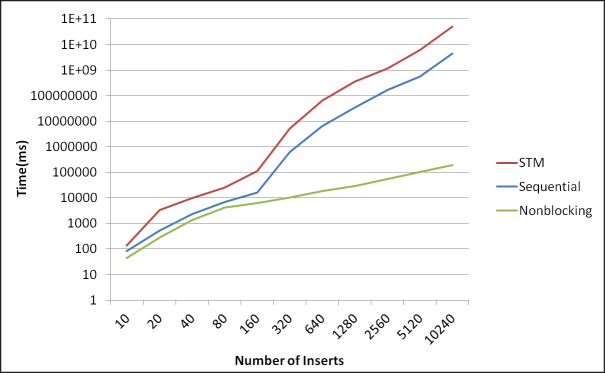
\includegraphics[width=0.45\textwidth]{insertTime.png}
Figure 2: Execution time vs. number of \textsc{Insert} operations for three implementations
\end{center}
\subsection{Lock Based}
TBD
\subsection{GCC Transactional Memory}
Here we have aimed to compare our non-blocking BST compared against the concurrent transactional memory-based BSTs. Here we used the GCCs built in support for atomic transactions. GCC provides a a facility where we can declare a fraction of code between following two labels ,
\STATE\_\_transaction\_atomic\_block\_starts
and \STATE\_\_transaction\_atomic\_block\_ends
, and GCC executes this fraction atomically, Readings for each configuration are averaged over 10 runs.  Concurrent transactional memory-based BST tests used $2^k$ threads in $k^{th}$ test case, with each thread inserting 10 random values.

\subsection{Syncrobench}
TBD

\section{Balancing}
Balancing is essential for maintaining efficient lookup in binary search trees -- after all, a pathologically unbalanced binary search tree is just a linked list.  Balancing ensures that access and update operations happen in $O(\log n)$ time rather than $O(n)$ time worst-case.

Sequential implementations of BSTs have taken several approaches to balancing.  In some cases, each update operation also takes care of balancing the tree (e.g. AVL tree rotations). However, this is not optimal in a highly parallel environment, because the internal structure of the tree is altered drastically on every update.  As a result, there are many more potential race conditions, and thus very few parts of the tree that can be trivially accessed concurrently.

In \cite{nurmi} Nurmi and Soisalon-Soininen discuss a lock-based approach for implementing chromatic trees, which are a variant of red-black trees with relaxed balancing constraints.  Their implementation decouples updates and balancing with an approach similar to the help functions used by Ellen et al. -- updating processes leave a record of contextual information that can be used by a separate balancing process.  There can be one or more balancing processes, and they can either run in the background concurrently with update processes during execution or can be invoked during downtime, similar to garbage collectors.  The authors focus on splitting the balancing operation into several small updates to minimize sequential bottlenecking. However, being a lock-based algorithm this proves not to be of much use.\\
Another approach for balancing an AVL tree is proposed in \cite{kessels}. There design is also allows insert and find operations only and is very similar to our implementation. Hence we have taken this approach for balancing.

\medskip


%Sets the bibliography style to ACM and imports the 
%bibliography file "ref.bib".
\bibliographystyle{acm}
\bibliography{ref}

\end{multicols}
\end{document}
% %%% Local Variables:
% %%% mode: latex
% %%% mode: flyspell
% %%% Local IspellDict: "american"
% %%% mode: outline-minor
% %%% End:
